\section{Overview on software testing}
Software testing is an essential part of the development process of a system, as it helps to ensure that a piece of software is reliable and performs as intended; it can be defined as the process of finding differences between the expected behavior specified by system's requirements and models, and the observed behavior of the implemented software. Unfortunately, it is impossible to completely test a nontrivial system. First, testing is not decidable. Second, testing must be performed under time and budget constraints \cite{OOSE}, therefore developers often compromise on testing activities by identifying only a critical subset of features to be tested.

There are many approaches to software testing, including unit testing, integration testing, system testing, as well as performance, penetration and acceptance testing. Each of these approaches has its own specific goals and methods, and they are often used in combination to ensure that a software product is thoroughly tested and conform to its specification.
\begin{itemize}
    \item \textbf{Unit Testing} is a method of testing individual units or components of a software product in isolation; its goal is to verify that each unit of code is working correctly and meets the specified requirements. Unit tests are typically written by the developers who wrote the code, and they are run automatically as part of the build process. Techniques also exist to generate input configuration for unit test automatically, by searching amongst the input space for the tests.
    \item \textbf{Integration Testing} is a method of testing how different units or components of a software product work together. The goal of integration testing is to ensure that the different parts of the system are integrated correctly and that they function as expected when combined. Integration tests are typically more complex than unit tests, as they involve multiple units of code working together.
    \item \textbf{System Testing} is a method of testing a complete software product in a simulated or real-world environment. The goal of system testing is to ensure that the software meets the specified requirements and performs as expected when running in a real-world environment. System tests may involve testing the software on different hardware or operating systems, or with different data inputs and configurations.
    \item \textbf{Acceptance Testing} is a method of testing a software product to ensure that it meets the needs and expectations of the end user. The goal of acceptance testing is to verify that the software is fit for its intended purpose and that it meets the requirements of the user. Acceptance tests are often written by the end user or a representative of the end user, and they may involve testing the software in a real-world environment
\end{itemize}


\subsection{Software Development Lifecycle}
Before discussing how testing activities are performed in more detail, it is essential to introduced how testing is integrated in the development process. The term Software Development Lifecycle, SDLC, refers to the entire process of developing and maintaining software systems. It includes the following phases:

\begin{figure}[h]
    \centering
    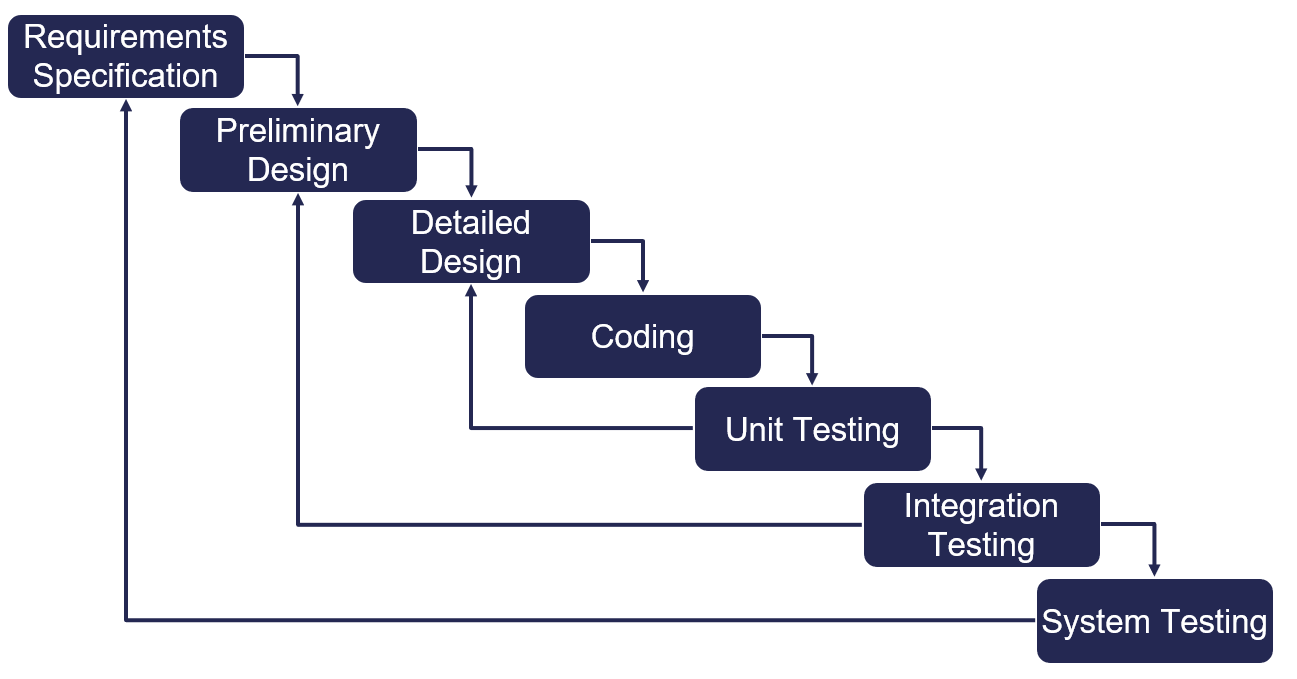
\includegraphics[width=\linewidth]{figures/waterfall_model.png}
    \caption{The Waterfall model}
    \label{waterfall_model}
\end{figure}

The main weakness of the Waterfall model is the very long feedback cycle between requirements specification and system testing; during this phase, the client is absent and there is no deliverable product before the end of the process

Modern software development strays away from non-incremental models, as today's applications are continuously evolving and adapting; instead

\begin{figure}[h]
    \centering
    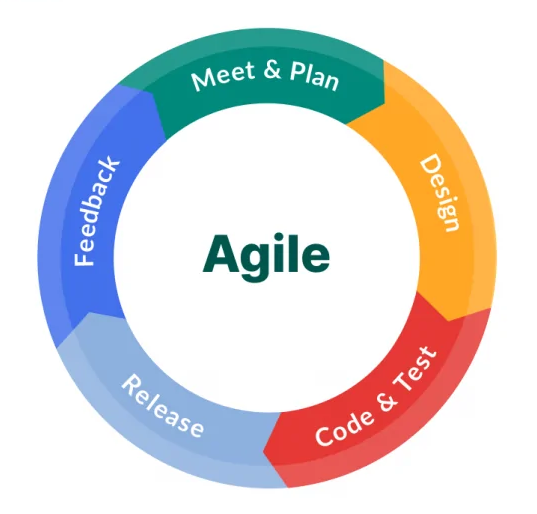
\includegraphics[width=\linewidth]{figures/agile_model.jpg}
    \caption{The Agile model}
    \label{agile_model}
\end{figure}



\section{Test Driven Development}

\subsection{Overview}
The concept of Test Driven Development (TDD) was firstly introduced in 2003 by Kent Back in the book "Test Driven Development By Example" \cite{TDDByExample}. While there is no formal definition of the process, as the author states, the goal is to "write clean code that works".
Compared to traditional SDL processes, TDD is an extremely short, incremental, and repetitive process, and is related to \textbf{test-first programming} concepts in extreme programming; this advocates for frequent updates/releases for the software, in short cycles, while encouraging code reviews, unit testing and incremental addition of features.


At its core, TDD is made up of three iterative phases: "Red", "Green" and "Blue" (or "Refactor"):
\begin{itemize}
    \item In the "\textbf{Red}" phase, a test case is written for the chunk of functionality to be implemented; since the corresponding logic does not exist yet, the test will obviously fail, often not even compiling.
    \item In the "\textbf{Green}" phase, only the code that is strictly required to make the test pass is written.
    \item Finally, in the "\textbf{Blue}" phase, the implemented code, as well as the respective test cases, is refactored and improved. It is important to perform regression testing after the refactoring to ensure that the changes didn't result in any unexpected behaviors in other components.
\end{itemize}
Each new unit of code requires a repetition of this cycle \cite{GuidelinesTDD}.

The figure below provides a representation of the TDD cycle:
\begin{figure}[h]
    \centering
    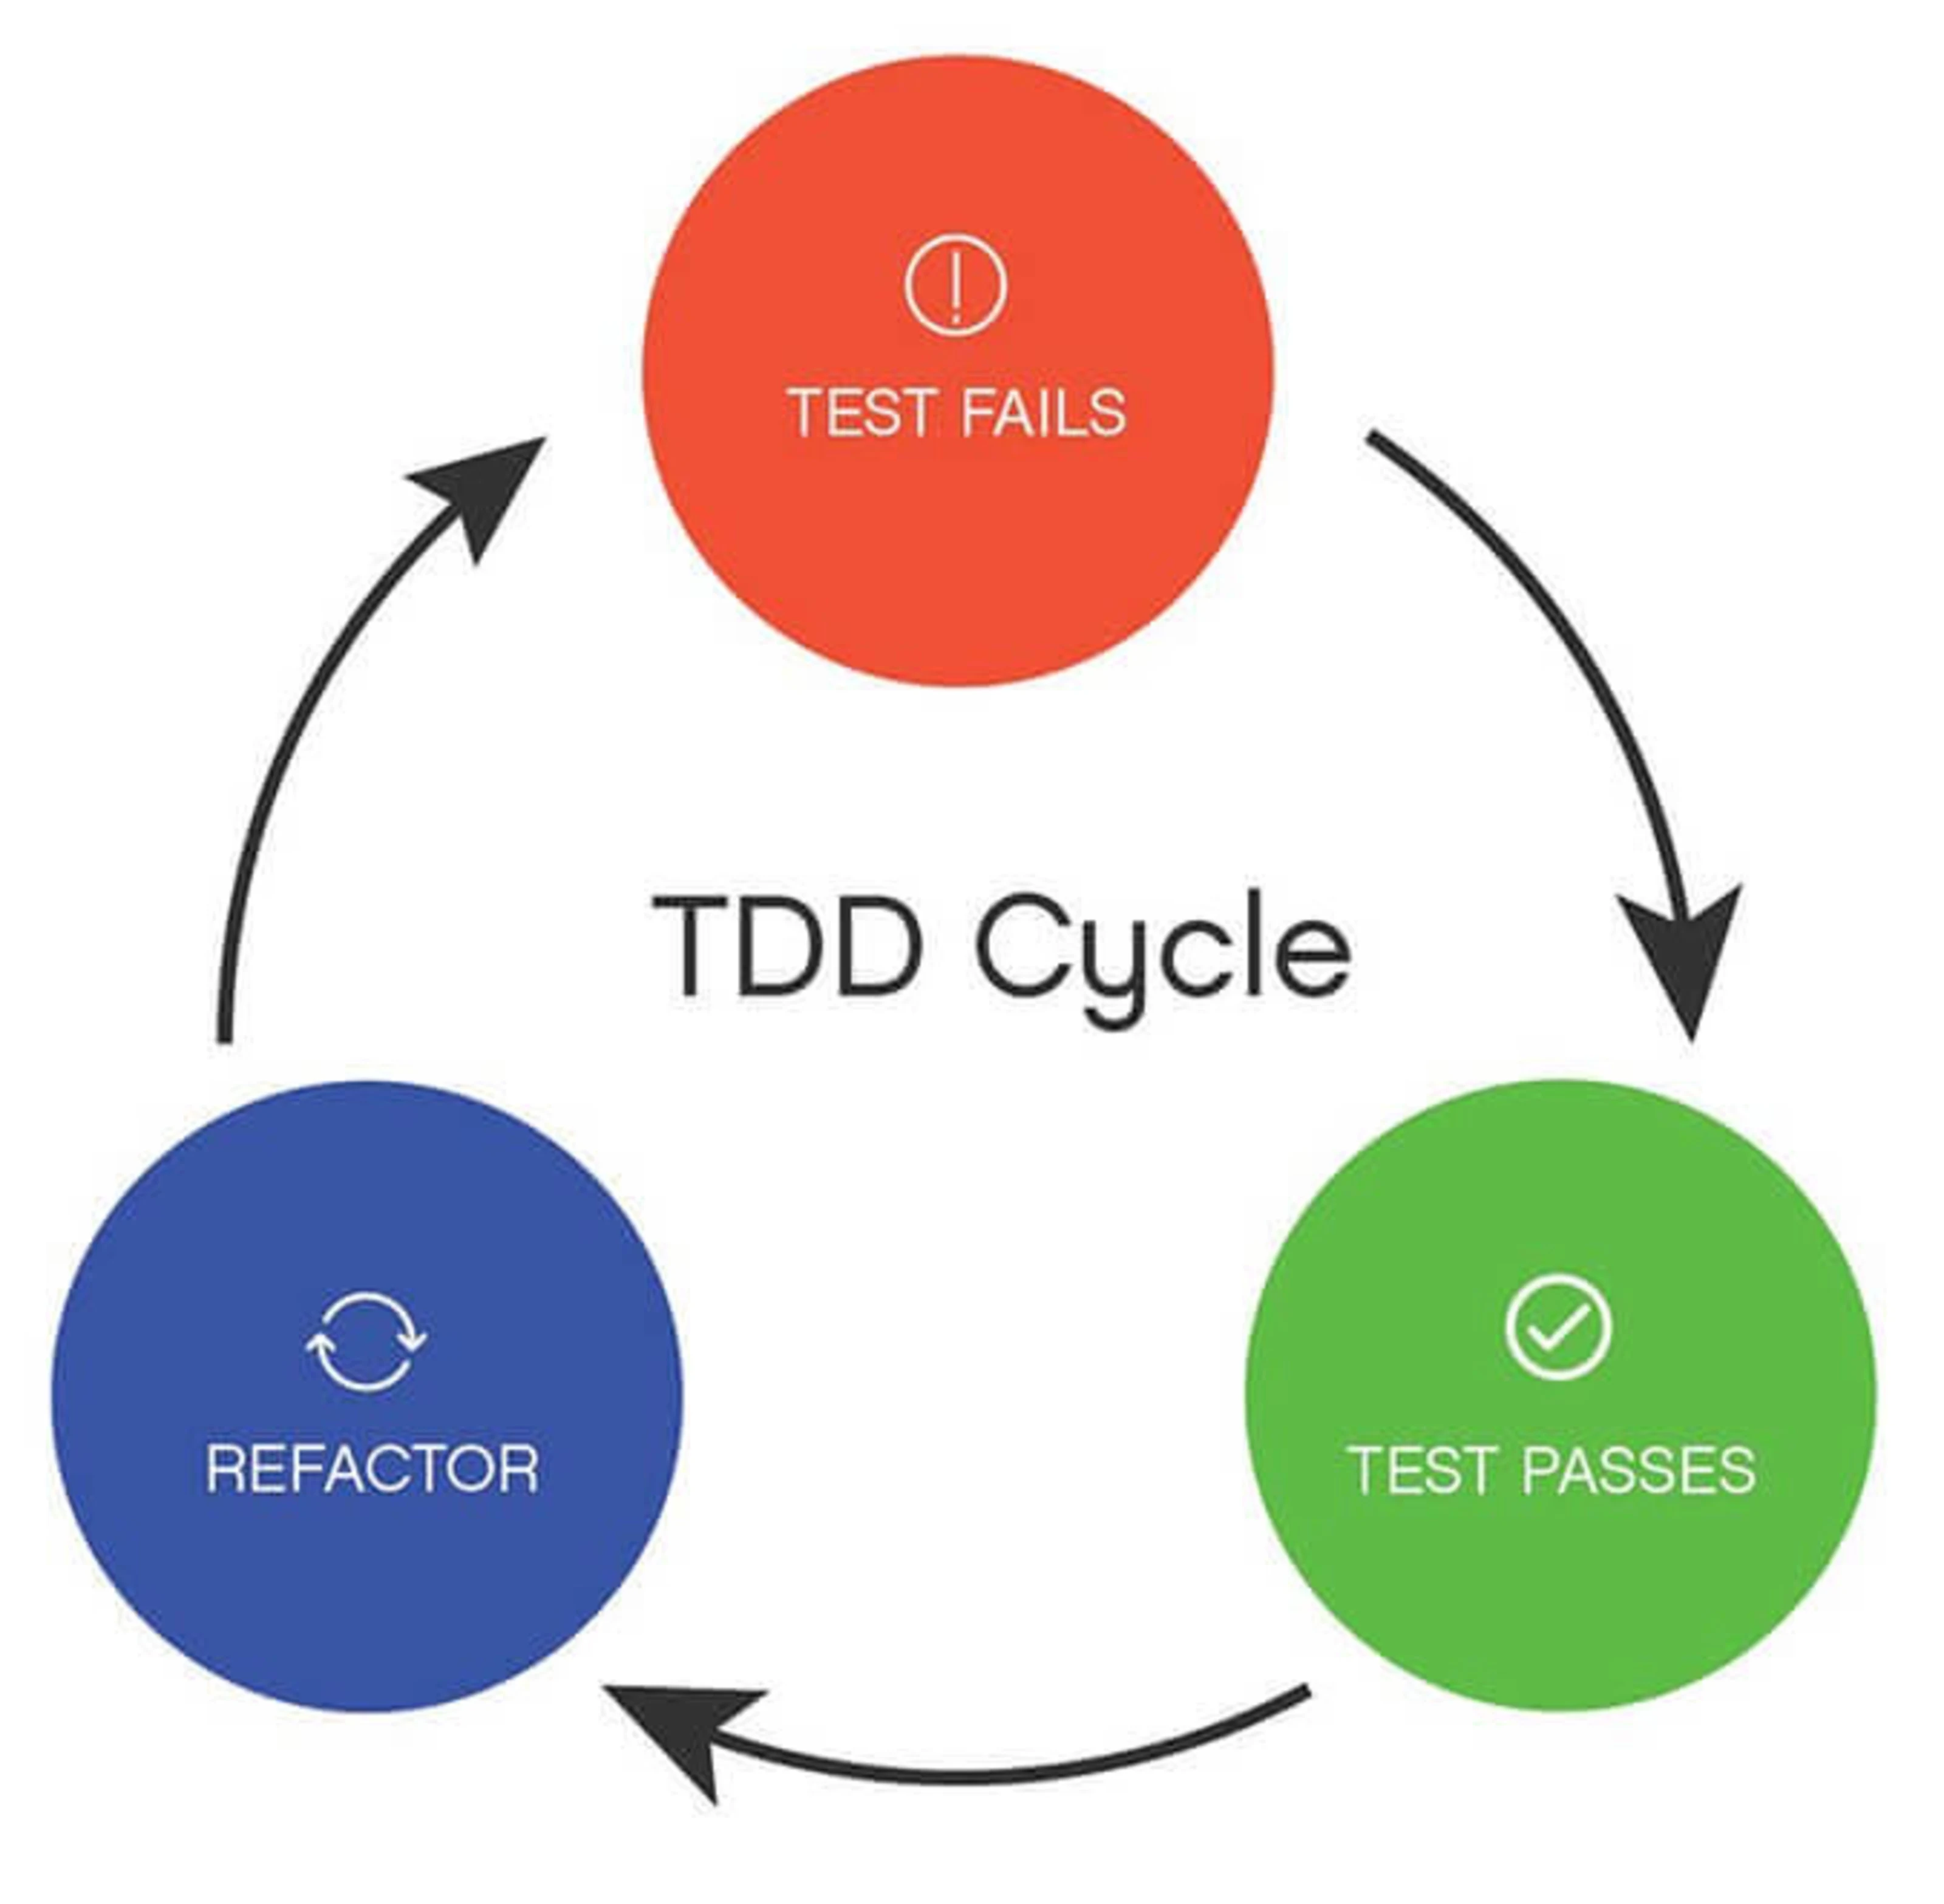
\includegraphics[width=\linewidth]{figures/tdd_cycle.jpg}
    \caption{The Test Driven Development cycle}
    \label{fig}
\end{figure}

As previously stated, each TDD iteration should be extremely short, usually spanning from 10 to 15 minutes at most \cite{}; this is possible thanks to a meticulous decomposition of the system's requirements into a set of \textbf{User Stories}, each detailing a small chunk of a functionality specified in the requirements. These stories can then be prioritized and implemented iteratively.

User stories can vary in granularity: when using a fine-grained structure when describing the task, this can be broken up into a set of sub-tasks, each corresponding to a small feature; on the other hand, with coarser-grained tasks, this division is less pronounced \cite{DBLP:journals/tse/KaracTJ21}. Even when the same task is considered, the outcome of the TDD process will change depending on the level of granularity employed when describing it; there is no overall right or wrong approach, rather it is something that comes from the experience of the developer to break tasks into small work items \cite{DBLP:journals/tse/KaracTJ21}.

The general mantra of TDD revolves around the "Make it green, then make it clean" motto

\subsection{TDD advantages}
The employment of TDD can result in a series of benefits during the development process, such as:
\begin{itemize}
    \item \textbf{Regression testing}: by incrementally building a test suite as the different iterations of TDD are performed, we ensure that the system  
    \item \textbf{Very high code coverage}: coverage is a metric used to determine how much of the code is being tested; it can be expressed according to different criteria such as statement coverage, i.e., how many statements in the code are reached by the test cases, branch coverage, i.e., how many conditional branches are executed during testing, or function coverage, i.e., how many functions are executed when running the test suite. While different coverage criteria result in different benefits, by employing TDD we ensure that any segment of code written has at least one associated test case.
    \item \textbf{Improved code quality}: as we are specifically writing code to pass the tests in place, and refactoring it after the "Green" phase, we ensure that the code is cleaner and overall more optimized, without any extra pieces of functionalities that may not be needed. 
    \item \textbf{Improved code readability and documentation}: test act as documentation...
    \item \textbf{Simplified debugging and early fault detection}: Whenever a test fails it becomes obvious which component has caused the fault: by adopting this incremental approach and performing regression testing, if a test fail we will be certain that the newly written code will be responsible. For this reason, faults are detected extremely early during the testing process, rather than potentially remaining hidden until the whole test suite has been built and executed.
\end{itemize}


